
%     %%%%%%%%%%%%%%%
%
%     P A C K A G E S
%
%     %%%%%%%%%%%%%%%

\documentclass[11pt, a4paper]{article}
\usepackage{fontspec}
\usepackage{caption}

% DOCUMENT LAYOUT
\usepackage{geometry}
\geometry{a4paper, textwidth=42em, textheight=70em, marginparsep=0.5em, marginparwidth=3.5em}
\setlength\parindent{0em}
\setlength\parskip{0.75em}
\captionsetup{width=0.8\textwidth}

% FONTS
\usepackage[usenames,dvipsnames]{xcolor}
\usepackage{xunicode}
\usepackage{xltxtra}
\defaultfontfeatures{Mapping=tex-text}
%\setromanfont [Ligatures={Common}, Numbers={OldStyle}, Variant=01]{Linux Libertine O}
%\setmonofont[Scale=0.8]{Monaco}
%%% modified by Karol Kozioł for ShareLaTeX use
\setmainfont[
  Ligatures={Common}, Numbers={OldStyle}, Variant=01,
  BoldFont=LinLibertine_RB.otf,
  ItalicFont=LinLibertine_RI.otf,
  BoldItalicFont=LinLibertine_RBI.otf
]{LinLibertine_R.otf}
\setmonofont[Scale=0.8]{DejaVuSansMono.ttf}

% HEADINGS
\usepackage{sectsty}
\usepackage[normalem]{ulem}
\sectionfont{\mdseries\upshape\Large}
\subsectionfont{\mdseries\scshape\normalsize}
\subsubsectionfont{\mdseries\upshape\large}

\renewenvironment{abstract}{%
{\mdseries\scshape\Large\abstractname}
\vspace{1em}\\
}{\par\noindent}

% LISTINGS
\usepackage{listings}
\usepackage{color}
\usepackage{appendix}

\usepackage{color}
\definecolor{codered}{rgb}{0.61,0.21,0.18}
\definecolor{codegreen}{rgb}{0,0.6,0}
\definecolor{codegray}{rgb}{0.5,0.5,0.5}
\definecolor{codepurple}{rgb}{0.58,0,0.82}
\definecolor{backcolour}{rgb}{1.0,1.0,1.0}
\lstset{
  backgroundcolor=\color{backcolour},   
  commentstyle=\color{codegray},
  keywordstyle=\color{codered},
  numberstyle=\tiny\color{codegreen},
  stringstyle=\color{codepurple},
  basicstyle=\footnotesize\ttfamily,        % the size of the fonts that are used for the code
  breaklines=true,                          % sets automatic line breaking
  keepspaces=true,                          % keeps spaces in text, useful for keeping indentation of code
  showspaces=false,                         % show spaces everywhere adding particular underscores; it overrides 'showstringspaces'
  showstringspaces=false,                   % underline spaces within strings only
  showtabs=false,                           % show tabs within strings adding particular underscores
  stepnumber=2,                             % the step between two line-numbers. If it's 1, each line will be numbered
  tabsize=2, 	                            % sets default tabsize to 2 spaces
  title=\lstname                            % show the filename of files included with \lstinputlisting
}


%     %%%%%%%%%%%%%%%
%
%     D O C U M E N T
%
%     %%%%%%%%%%%%%%%


\begin{document}
\title{IAR Task 1 Report}
\author{Angus Pearson -- s1311631\\ Jevgenij Zubovskij -- s1346981}
\date{\today}
\maketitle

%       ^v^v^v^v^v^v^v^v^v^v^v^v^v^v^v^v^v^v^v^v^v^v^v^v^v^v^v^v^v^v^v^v^v^v^v^


\begin{abstract}
  We have implemented a control program for the Khepera robot, utilising eight IR distance
  sensors to reactively avoid colliding with obstacles, follow the perimeter of an object 
  or wall  and explore the environment. Multiple avenues of control were investigated and 
  compared. The notion of the robot becoming bored affords interesting behaviours and an 
  enhanced ability to explore an environment. The prominent limitations are the robot's 
  sensing suite, with a small number of sensors and artefacts arising from the physics 
  of IR sensing.
\end{abstract}

%       ^v^v^v^v^v^v^v^v^v^v^v^v^v^v^v^v^v^v^v^v^v^v^v^v^v^v^v^v^v^v^v^v^v^v^v^


\section{Introduction}

The first assignment entails utilising infra-red distance sensors on the Khepera 
robot to navigate autonomously around an environment, ``without hitting obstacles 
or getting stuck in corners or dead-ends. Second, the Robot should tend to follow long walls, 
keeping a consistent distance away from the wall.'' The Robot is controlled remotely 
 by a computer over serial. We have elected to use Python as the 
implementation language for this practical.

As per the Task description, we split the development into two goals, one being obstacle 
avoidance and the other being a wall-following behaviour. Our approach is influenced 
by the demonstrable abilities of reaction-based control in robotics and the BUG 
algorithms \cite{principlesrobot}.

%       ^v^v^v^v^v^v^v^v^v^v^v^v^v^v^v^v^v^v^v^v^v^v^v^v^v^v^v^v^v^v^v^v^v^v^v^


\section{Exploring Methods of Not Hitting Things}

\subsection{Experimenting with PID}

An 8-dimensional PID controller was implemented over the sensor data, yielding an error 
with respect to the distance from an obstacle per sensor -- Too far, the error motivates 
a movement towards the object; Too close and the error motivates a move away.

The approach had some promising behaviours: The robot was able to avoid hitting an object.
However, wall following would either oscillate towards the wall, bumping against it or 
depart after following for a short distance. This is due in part to the narrow field 
of view afforded by solely using the forward-facing sensor pair.

However the controller was very sensitive to it's tuned gains ${K_p}$, ${K_i}$ \&
${K_d}$ and tended to perform best when ${K_p}$ was much larger than the other gains.
The control is neither continuous nor low-latency, as we used discrete thresholds to 
react to the error vector PID produced. Thus, we discard PID in favour 
of a simpler reactive solution.


\subsection{Force-Vector Control}

We consider treating each distance sensor reading as a force vector pushing 
the robot along the axis of it's sensor. Summing these forces gives us an 
`Intended Direction' resultant vector, which is used to correct the initial 
direction vector away from the obstacle.

\begin{figure}[h]
  \begin{center}
    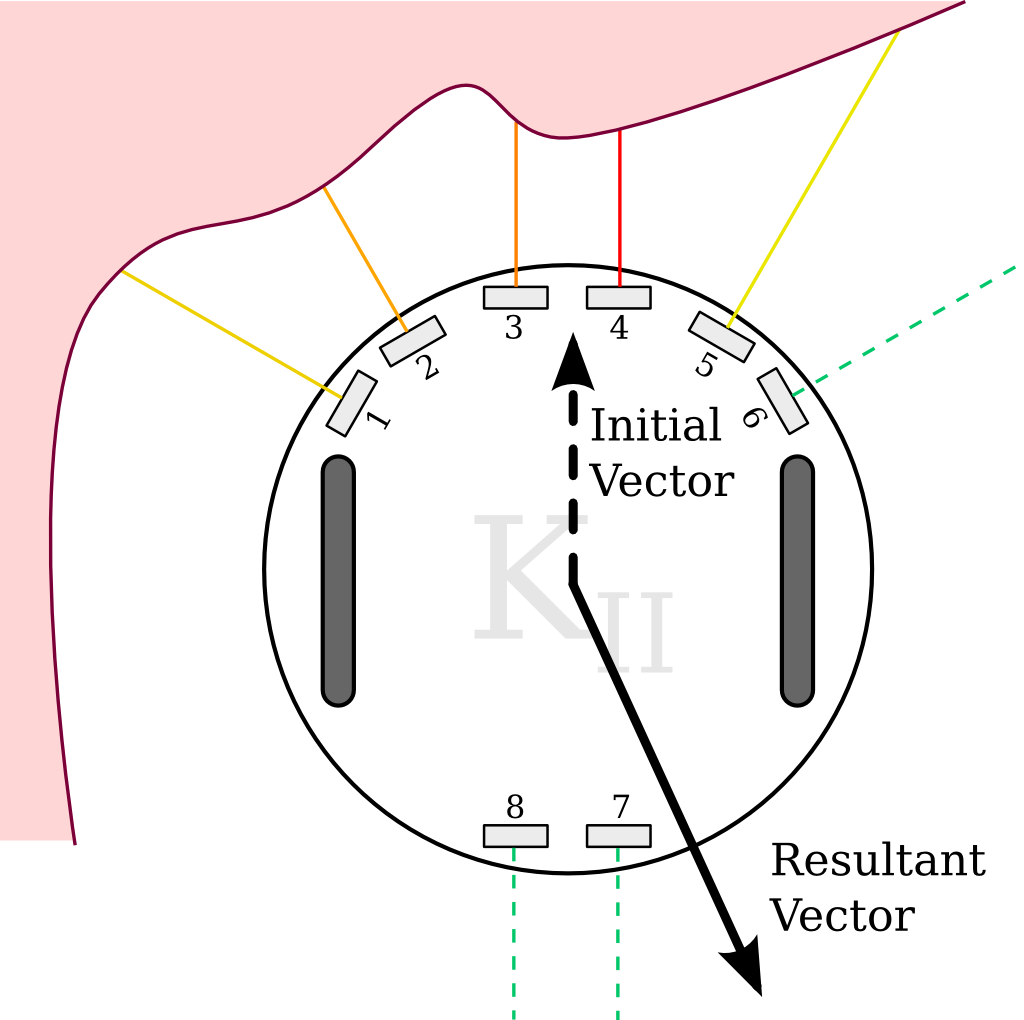
\includegraphics[width=18em]{../assets/force-vector.png}
    \caption{Showing the derivation of Force Vector from distance readings to the
      obstacle; A shorter distance to the obstacle yields a stronger push in the 
      opposite direction. Distances over a threshold (shown dashed) are ignored 
      and have magnitude $0$.}
  \end{center}
\end{figure}

Experimentation showed that the lack of calibration between sensors and 
direct mapping to forces introduced a `wobble', with no exhibition of 
wall-following as the error vectors push in direct opposition to the wall, 
resulting in the robot basically bouncing off. Attempts to smooth or condition the 
sensor signals to prevent wobbling gave the robot poor performance in any environment 
with sharp angles.

The method is somewhat more elegant than PID \& rule based control insofar 
as the complexity of behaviour that emerges from a simple rule set. Nonetheless, we 
discard Force-Vector control in favour of Reaction-Based control using some methods 
learned from the PID Experiment.

%       ^v^v^v^v^v^v^v^v^v^v^v^v^v^v^v^v^v^v^v^v^v^v^v^v^v^v^v^v^v^v^v^v^v^v^v^


\section{Developing Object-Following Behaviour}

It was decided to build upon threshold based avoidance control. However, 
that would require an algorithm that accounts for the robot not being intrinsically
able to keep a  \emph{at a constant distance} from a wall.

Thus, final obstacle-avoidance method reactionally adjusts our trajectory away from a 
collision using a composition of multiple distance sensors, using different groups to 
decide first whether an obstacle is too close, then deciding which way to turn using 
the sensors to choose a direction that presents a larger open-space to move into.
Discrete thresholds are used to make decisions about closeness. When we have made a 
decision to rotate left or right we stick with it until the forward direction is clear; 
this prevents an indecisive oscillation and the robot becoming stuck. We make no 
distinction between a wall and another shape.

\subsection{Sensor Use}

Different scaling is applied to sensors on the side of the robot than the front, as we 
can afford to be closer to an obstacle when travelling parallel to it rather than 
when perpendicularly approaching (Given the robot always moves forwards). Please 
see the code for more detailed implementation explanation. The outline of sensor use in 
the control loop is as follows:

\begin{enumerate}

	\item Sensors ($0$, $1$, $2$, $3$, $4$, $5$) used to determine if robot can no longer proceed in the 
forward direction and which way we have more space to move and, hence, should unstuck towards.

	\item Sensors ($1$, $2$, $3$, $4$) to detect followable shape and what side of the robot (left / right) to follow it on. 

	\item Sensors ($0$, $5$) used to ensure we follow the shape within a consitent range of values

	\item The back sensors ($6$, $7$) were not used due to our robot only moving in the forward direction 
and 6 sensors allowing better control than 2

\end{enumerate}

\subsection{Boredom, a useful concept}

The notion that the robot may become `bored' with a wall that it is pursuing gives 
rise to some useful behaviours: An intrinsic property of becoming bored with a wall 
is that we will not forever circle an obstacle thinking it is just a really long wall. 
This also gives the robot a much higher chance of fully exploring it's environment 
given enough time, as random changes in course will continuously occur.

We implemented a boredom algorithm, counting how long a wall has been followed for without interruption (being stuck).

\section{Algorithm}

Every 20 ms a control loop iteration starts by taking new IR measurements. The 20 ms delay is used 
in order for the IR sensors to update between iterations. The IR data is then used 
determine further actions in descending order of priority:

\begin{enumerate}
  \item If the robot is ``bored'' it begins a set of cycles to turn away from the followed shape 

  \item If robot is finished turning away from ``boring'' wall, it drives forward until it becomes stuck when the loop resumes from ${3.}$

  \item If the robot is stuck and cannot continue moving in the frontal direction, then it turns in the direction away from the previously followed shape or towards where the sensors detected more space until it detects it is no longer stuck. 

  \item If the robot encounters (or was previously following) a shape it can follow, it follows it on either left or right side (depending to which one is closer) at a consistent distance perpendicular to the shape's edge.
  
  \item If robot has just initialized or has nothing else to do, it drives forwards until $3$ or $4$ occur. 
\end{enumerate}

The following is a representation of the algorithm in a state diagram form:
\begin{figure}[h]
  \begin{center}
    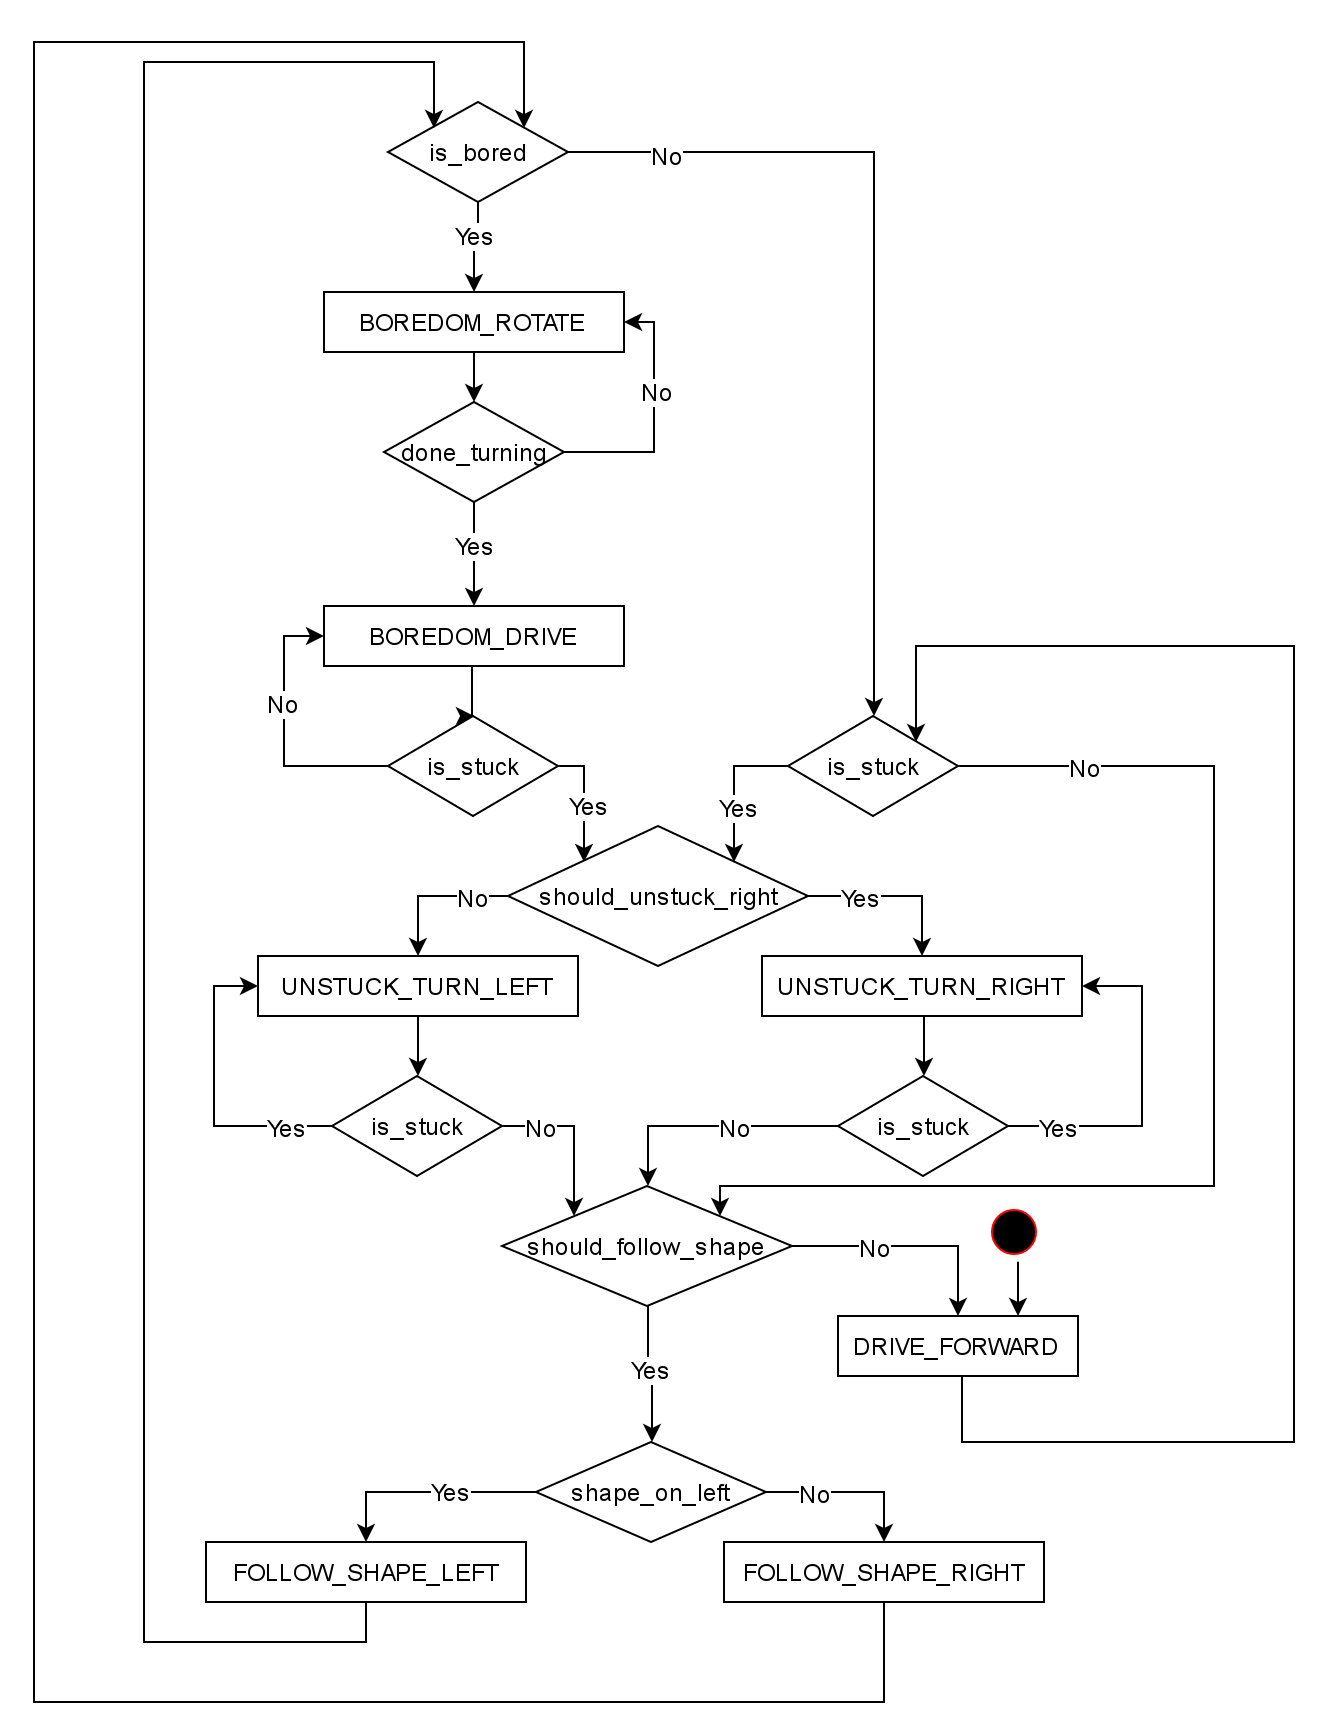
\includegraphics[width=30em]{../assets/state-diagram.png}
    \caption{Illustration of the algorithm in a state diagram form.}
  \end{center}
\end{figure}

\begin{center}
  \emph{Source Code is included in the Appendix.}
\end{center}



Direct reactionary control multiply motor speed by error for that side

%       ^v^v^v^v^v^v^v^v^v^v^v^v^v^v^v^v^v^v^v^v^v^v^v^v^v^v^v^v^v^v^v^v^v^v^v^

\newpage
\section{Results}

The robot is able to follow any shape it encounters at a close distances and 
avoid getting stuck among obstacles, dead ends and mazes. Moreover, it exhibits 
exploratory behavior due to the boredom concept implemented. However, it approached
the outlines of darker objects noticeably closer than that of lighter ones 
even after several rounds of calibrating the thresholds.


\section{Discussion \& Possible Improvements}

The chosen method and algorithm proved successful. The system works as
per requirements and has an emergent, seemingly intelligent behavior by navigating and 
exploring the environment. However, physical capabilities were not fully utilized
as back sensors are not used and movement is only in the forward direction. 


Darker objects absorb more light, reaching the threshold IR value at a considerably closer 
distance than lighter ones. The algortihm does not discriminate, meaning darker objects are 
followed at a closer distance than lighter ones as same threshold value is used. Thus, a 
method allowing differentiation would allow equal distances to be held from all objects 
regardless of their absorbant properties. 


\section{Physical Limitations and Possible Improvements}

The Khepera's distance sensors are spaced to prioritise forward motion, which is beneficial 
for exploring a space though does make reversing out of a dead-end much harder than 
turning on the spot then driving out forwards. Evenly spaced sensors in all directions would 
allow better estimation of object positions.

Moreover, a bump (or other touch) sensor would allow easier detection of collisions and 
obstacles in case the IR sensor based algorithms fails to detect or predict an object.


%       ^v^v^v^v^v^v^v^v^v^v^v^v^v^v^v^v^v^v^v^v^v^v^v^v^v^v^v^v^v^v^v^v^v^v^v^

\begin{appendices}
\section*{Appendix}
\subsection{Code Listings}
\lstinputlisting[language=python]{../../main.py}
\lstinputlisting[language=python]{../../comms.py}
\lstinputlisting[language=python]{../../constants.py}
\end{appendices}


\begin{thebibliography}{1}

\bibitem{principlesrobot}
Principles of Robot Motion: Theory, Algorithms, and Implementation\\
\textit{Howie Choset}

\end{thebibliography}
\end{document}
